\documentclass[12pt]{article}

\usepackage{amsmath,amssymb,amsthm}
\usepackage[T1]{fontenc}
\usepackage{graphics}
\usepackage{qtree}
\usepackage{tikz}
\usepackage[utf8]{inputenc} % æøå
\usepackage[T1]{fontenc} % mere æøå
\usepackage[danish]{babel} % orddeling
\usepackage{verbatim} % så man kan skrive ren tekst
\usepackage[all]{xy} % den sidste (avancerede) formel i dokumentet
\usepackage{fullpage} % mindre margin

\title{PKSU - Props 2.0}
\author{Louise Knudsen, Helena Bach, David Pedersen}
\date{\today}

\newcommand{\R}{\mathbb{R}}
\newcommand{\C}{\mathbb{C}}
\newcommand{\N}{\mathbb{N}}
\newcommand{\Z}{\mathbb{Z}}
\newcommand{\Q}{\mathbb{Q}}

\newcommand{\og}{\wedge}

\begin{document}
\maketitle
\section{Problem definition}
\textit{The Royal Danish Theatre's props department uses a locally installed database-system to search through all of the props and productions and their corresponding set-up- and run-lists. The system was developed more than 20 years ago by their own Claus Nepper Fakkenberg. Claus alone holds the responsibility for maintaining the system, as he is the only one who understands the source-code, which will soon be a problem as he is now retiring. \\
Due to the age of the system, some functionalities are no longer needed, and there are new requirements that are not implemented, most importantly a need to use the system outside of the office.} \\\\
The problem can be described with the following points:
\begin{itemize}
\item The current database system was developed in 1989, and lacks a lot of wanted functionalities.
\item The developer, Claus, is the only one who can modify and support the system.
\item Claus is retiring.
\end{itemize}
To analyze the problems defined above and develop a system definition we use the FACTOR Criterion.
\subsection{The FACTOR Criterion}
\begin{description}
  \item[Functionality:] Keeping track of the props and performances, and help in running these. As well as support the administration.
  \item[Application domain:] The Royal Danish Theatre.
  \item[Conditions:] The system should be usable by multiple user at a time, wherever there are access to the internet.
  \item[Technology:] The system will be developed on standard laptops, and should be usable on standard PC's and tablets and supported by every OS.
  \item[Object:] Props, pictures and employees in the props department.
  \item[Responsibility:] Searching and administrative tool.
\end{description}
\subsection{System definition}
A web-based database-system of The Royal Danish Theatre props department. The system should primarily be a searching tool used to prepare and run performances and search for props in current and previous productions by the assistant stage managers, and secondly be used for budget monitoring, search for supplier information as well as keeping track of all performance information, by the chairman of the props department. The system should be usable for people with greatly variable computer experience.
\subsection{Requirements}
We have had multiple meetings with the different people who have daily contact with the system to form a idea of the needs and requirements, but only April 9th these will be formalised more specifically, when we kick off the project in collaboration with the client.
\subsection{Constraints}
The constraints of our project include the security aspect, which the head of the IT-department, Martin Thaarup Larsen, makes sure to handle in a way that makes it possible for our system to be part of the existing login-system. Martin has the responsibility for the media database as well - most likely made accessible to us through a "mirror database".   
\subsection{Solution domain}
The solution domain can be defined as being the props department as well as Cumulus, their media database, which our application will be interfacing with.
\subsection{Deliverables}
- PHP code \\
- MySQL database \\
- Instructions in the form of meetings in addition to papers explaining the system.\\
- Probably also some support during the initial start up phase.
\section{Initial Software Project Management Plan}
\subsection{Overview of the project}
To give a initial overview of the project in terms of planning and managing we have composed the following points.
\subsubsection{Project summary}
\underline{Work product:} \\
- MySQL database \\
- PHP code for the web-interface. \\
- Assignments describing the work process\\\\
\underline{Schedule:} \\
On April 9th we are scheduled to meet with Martin and Mikkel from the theatre, to finalize the requirements elicitation and sign the project agreement. We will thereafter be able to put together a more detailed time-schedule.\\
On June 23rd we have our final deadline, and will hopefully deliver the final product to the theatre. \\\\
\underline{Participants:}\\
Developers: David Pedersen, Helena Bach, Louise Knudsen \\
Project managers: David Pedersen, Helena Bach, Louise Knudsen \\
Client: The Royal Danish Theatre.\\\\
\underline{Tasks:} \\
The developers will have a common responsibility to participate in every aspect of the system-development. Of course their will be a natural division of the task in correspondence to each developers skill- and interest-level as described in the skill matrix, which is found in section 5. 
\subsubsection{Evolution of the plan}
All changes to the project management plan must be agreed to by all participants before they are implemented. All changes should be documented in the, to the developers, shared log, and in time become a part of the final SPMP.
\subsection{References}
All artifacts will conform to the theatres standards.
% TODO: noget med PHP og mySQL??
\subsection{Definitions}
The Royal Danish Theatre uses a lot of different terms in their work, and some of these should also be used in the future database system. The terms we have been presented to so far are listed with a short description below: \\
Every production has a unique 8-digit number, containing of 4 random digits followed by a dash and premiere-year for this particular production. (There can be multiple productions of, for instance the same play, which then have different premiere-years) \\
If a production is \textit{SKILT}, it means that it has been discarded and the props are back in the storage room. \\
If a production is \textit{I REPERTOIRE}, it is being played in the current season and the props are in use. \\
If the production is \textit{I CONTAINER} or similar, the production is not yet \textit{SKILT} nor is it currently being played, and the props are therefore occupied but not in use.
\subsection{Project Organization}
\subsubsection{External interfaces}
The props database and appertaining web-interface will be managed and developed by David Pedersen, Helena Bach and Louise Knudsen. \\
The photographs of the props and productions, along with the login system and server connection will be handled by Martin. \\
All managers will be in continuous contact with the chairman of the props department, Mikkel Rasmus Theut, as well as Martin. 
%\subsubsection{Internal structure}
%Skal vi have den her med? det samme som partisipants?
%\subsubsection{Roles and responsibilities}
% TODO: Noget med opdeling af arbejdet. noget med skill matrix: David 1 i web, Helena og Louise 1 i DB?? Alle vil være indover alle opgaver, men David har ansvaret for web, Helena og Louise for DB?????
\subsection{Managerial process plans}
\subsubsection{Start-up plan}
The total developments time is estimated to be 15 week, counting from 13/03/2014, where first meeting with the client were held. \\
% TODO: Noget med roller i løbet af processen. \\
All necessary hardware are available, as well are the software since MySQL and PHP both are open-source.
\subsubsection{Work plan}
\underline{Week 1-5:}
\begin{itemize}
\item Initial meeting with Mikkel.
\item More technically oriented meeting with Martin where Mikkel were also present.
\item Meeting with head of the furniture subdivision.
Prepare the requirements elicitation and the Project Agreement.
\item Meeting with Martin and Mikkel - signing of the requirements elicitation and the Project Agreement, and project kick-off!
\end{itemize}
\underline{Week 6-7:}
\begin{itemize}
\item Focus on making the SQL-script.
\end{itemize}
\underline{Week 8-11:}
\begin{itemize}
\item Finish SQL.
\item Start design of the web-application.
\item Begin PHP-coding and testing.
\end{itemize}
\underline{Week 12-15:}
\begin{itemize}
\item Finish PHP-coding and testing.
\item Final documentation.
\end{itemize}
%\subsubsection{Control plan}
% TODO: Noget i forhold til Roles/responsibilities, med at David har ansvaret for Web, og Helena og Louise har for DB. Vi har fælles ansvar for dokumentation. Dette sker med intern kontakt mindst 2 gange ugenligt.
\subsubsection{Risk management plan}
The risk factors and the tracking mechanisms are as follows. \\\\
As one of the goals of the project is to achieve more functionality than the existing system, there should in the testing-process be compared results between the two. \\\\
There should in the designing-process be a great amount of communication with the client to ensure an as user-friendly interface as possible, as the system mainly will be used by people with limited computer-experience. \\\\
There is a slim chance of hardware failure, in which case each developer is responsible for there own computer, and the client holds the responsibility for the server. \\\\
Each developer is responsible for continuous testing of their assigned subsystem(s) and jointly cross-testing between these. 
%\subsubsection{Closeout plan}
% TODO: noget ????
\subsection{Techinical process plans}
% TODO: noget med kap 15...
\subsubsection{Process model}
\subsubsection{Methods, tools, and techniques}
\subsubsection{Infrastructure}
\subsubsection{Product acceptance plan}
\subsection{Supporting process plans}
\subsubsection{Configuration management plan}
Git and GitHub will be used in all aspects of the project to ensure version control.
\subsubsection{Verification and validation plan}
% TODO: noget med test ift. 6'eren.
\subsubsection{Documentation plan}
% TODO: måske noget med loggen, og PHP-Doc?
\subsubsection{Quality assurance plan}
% TODO: noget???
\subsubsection{Reviews and audits}
??
\subsubsection{Problem resolution plan}
\subsubsection{Subcontractor management plan}
\subsubsection{Process improvement plan}
\subsection{Additional plans}
\subsubsection{Presentation}
In connection with the delivery of the final product, the system and its functionalities will be a presented to the chairman of the props department, Mikkel. \\
As one of the purposes of developing the new system, is to make it possible for the head of the IT-department, Martin, to keep the system up to date himself, we will in addition to the presentation, be going through code with him.
\subsubsection{Support}
During the initialisation phase support will be offered free of charge.
\section{Initial software architecture}
\section{Project Agreement definition}
As mentioned in previous sections our final requirement elicitation and project agreement will be formalized on April 9th, at our meeting with Mikkel and Martin. To prepare for the meeting and make an outline for this final definition we have made the following UML use case diagram (See Appendix X for use cases) and functional/nonfuntional requirements overview.
\subsection{UML use case diagram}
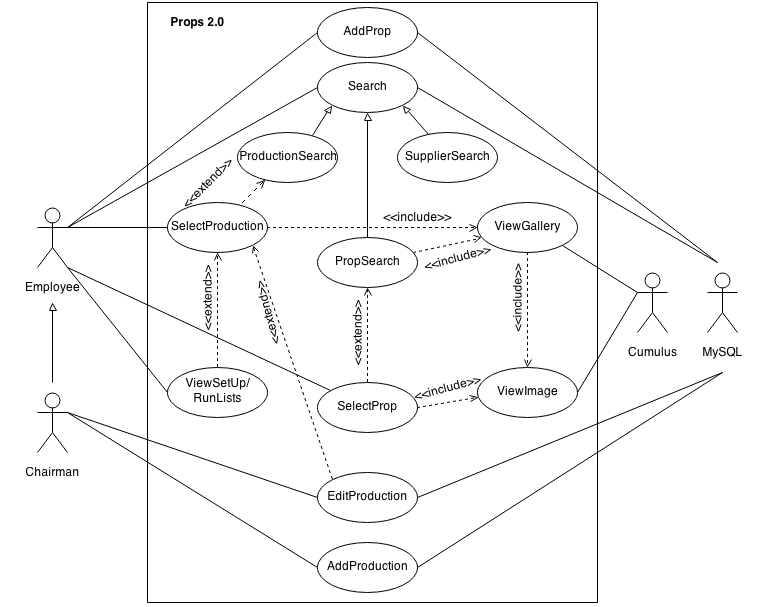
\includegraphics[scale=0.6]{use.png}
\subsection{Nonfunctional Requirements}
\begin{itemize}
\item The system should be web-based and usable on standard PC's and tablets, and supported by every OS.
\item The webapplication should be user friendly and easy to navigate. The most commonly used functionalities, namely the run- and set-up-lists should not be more than 3 clicks away.
\item It should be possible for Martin to maintain and support, and possibly expand the system after product-delivery. Therefore the system will be developed using MySQL and PHP, which is familiar to the XX.
\item The system should be able to communicate with the existing media-database Cumulus.
\item noget med firewall login og halløj.
\item The interface should be in Danish.
\end{itemize}
\subsection{Functional Requirements}
\begin{itemize}
\item It should be possible to do cross search for props, productions and suppliers.
\item It should be possible to add, edit and delete props, productions and suppliers.
\item noget med Kongeplanen
\item It should be possible to print run- and set-up-lists.
\item noget med drag/drop props til run- and set-up-lists.
\end{itemize}
\subsection{Use cases}
%1. Tilføj Rek
\[
\begin{array}{ll}
\hline
\textit{Use case name} & \texttt{AddProp} \\
\hline
\textit{Participating actors} & \text{Initiated by \texttt{Employee}} \\
& \text{Communicates with \texttt{MySQL}} \\
\hline
\textit{Flow of events} & 
\begin{array}{l}
\text{1. The \texttt{Employee} activates the "Add prop"  function.}\\
\quad \quad \quad \text{2. \texttt{Props 2.0} responds by presenting a form to the \texttt{Employee}.} \\
\text{3. The \texttt{Employee} fills out the form with the relevant prop-info,} \\ \quad \text{and submits it.} \\
\quad \quad \quad \text{4. \texttt{Props 2.0} receives the form, and the MySQL database} \\ \quad \quad \quad \quad \text{gets updated. \texttt{Props 2.0} displays a confirmation of the}\\ \quad \quad \quad \quad \text{update.}
\end{array} \\
\hline
\textit{Entry condition} & \text{The \texttt{Employee} must be logged into the Theatre's Wi-Fi} \\
\hline
\textit{Exit condition} & \text{The \texttt{Employee} has received a confirmation OR} \\ & \text{An explanation indicating why the transaction could not be processed.} \\
\hline
\textit{Quality requirements} & \text{Not yet defined} \\
\hline
\end{array}
\]
%2. Tilføj forestilling
\[
\begin{array}{ll}
\hline
\textit{Use case name} & \texttt{AddProduction} \\
\hline
\textit{Participating actors} & \text{Initiated by \texttt{Chairman}} \\
& \text{Communicates with \texttt{MySQL}} \\
\hline
\textit{Flow of events} & 
\begin{array}{l}
\text{1. The \texttt{Chairman} activates the "Add production" function.}\\
\quad \quad \quad \text{2. \texttt{Props 2.0} responds by presenting a form to the \texttt{Chairman}.} \\
\text{3. The \texttt{Chairman} fills out the form with the relevant production-info,} \\ \quad \text{and submits it.} \\
\quad \quad \quad \text{4. \texttt{Props 2.0} receives the form, and the MySQL database} \\ \quad \quad \quad \quad \text{gets updated. \texttt{Props 2.0} displays a confirmation of the}\\ \quad \quad \quad \quad \text{update.}
\end{array} \\
\hline
\textit{Entry condition} & \text{The \texttt{Chairman} must be logged into the Theatre's Wi-Fi} \\
\hline
\textit{Exit condition} & \text{The \texttt{Chairman} has received a confirmation OR} \\ & \text{An explanation indicating why the transaction could not be processed.} \\
\hline
\textit{Quality requirements} & \text{Not yet defined}\\
\hline
\end{array}
\]
%3. Søg
\[
\begin{array}{ll}
\hline
\textit{Use case name} & \texttt{Search} \\
\hline
\textit{Participating actors} & \text{Initiated by \texttt{Employee}} \\
& \text{Communicates with \texttt{MySQL}} \\
\hline
\textit{Flow of events} & 
\begin{array}{l}
\text{1. The \texttt{Employee} activates the "Search" function.}\\
\quad \quad \quad \text{2. \texttt{Props 2.0} responds by presenting a form to the \texttt{Employee}.} \\
\text{3. The \texttt{Employee} fills out the form with the search criteria,} \\ \quad \text{and submits it.} \\
\quad \quad \quad \text{4. \texttt{Props 2.0} receives the form, the MySQL database} \\ \quad \quad \quad \quad \text{returns the matching data and \texttt{Props 2.0} displays it}
\end{array} \\
\hline
\textit{Entry condition} & \text{The \texttt{Employee} must be logged into the Theatre's Wi-Fi} \\
\hline
\textit{Exit condition} & \text{The \texttt{Employee} has received a list of matching data OR} \\ & \text{A "No match"  message} \\
\hline
\textit{Quality requirements} & \text{Not yet defined} \\
\hline
\end{array}
\]
We have not yet fully specified the search criteria with client. We know that separate search-functions for productions, props and suppliers are wanted, but until we have the detailed criteria, we will not include these as specific use cases.  
%4. Vælg rek
\[
\begin{array}{ll}
\hline
\textit{Use case name} & \texttt{SelectProp} \\
\hline
\textit{Participating actors} & \text{Initiated by \texttt{Employee}} \\
\hline
\textit{Flow of events} & 
\begin{array}{l}
\text{1. The \texttt{Employee} selects a prop from the results of a premade search} \\
\quad \quad \quad \text{2. \texttt{Props 2.0} responds by presenting a more detailed}\\ \quad \quad \quad \quad \text{description of the prop to the \texttt{Employee}.}
\end{array} \\
\hline
\textit{Entry condition} & \text{This use case extends the  \texttt{PropSearch} use case} \\
\hline
\textit{Exit condition} & \text{The \texttt{Employee} is looking at the prop description} \\
\hline
\textit{Quality requirements} & \text{This use case includes the \texttt{ViewImage} use case} \\
\hline
\end{array}
\]
%5. Vælg forestilling:\\
\[
\begin{array}{ll}
\hline
\textit{Use case name} & \texttt{SelectProduction} \\
\hline
\textit{Participating actors} & \text{Initiated by \texttt{Employee}} \\
\hline
\textit{Flow of events} & 
\begin{array}{l}
\text{1. The \texttt{Employee} selects a production from the results of a premade}\\ \quad \text{search}\\
\quad \quad \quad \text{2. \texttt{Props 2.0} responds by presenting a more detailed}\\
\quad \quad \quad \quad \text{description of the production to the \texttt{Employee}.}
\end{array} \\
\hline
\textit{Entry condition} &
\text{This use case extends the \texttt{ProductionSearch} use case.}\\
\hline
\textit{Exit condition} & \text{The \texttt{Employee} is looking at the production information.} \\
\hline
\textit{Quality requirements} & \text{This use case includes the \texttt{ViewGallery} use case.} \\
\hline
\end{array}
\]
%6. Køre/opstil
\[
\begin{array}{ll}
\hline
\textit{Use case name} & \texttt{ViewSetUp/RunLists} \\
\hline
\textit{Participating actors} & \text{Initiated by \texttt{Employee}} \\
\hline
\textit{Flow of events} & 
\begin{array}{l}
\text{1. The \texttt{Employee} selects the list from the results of a production} \\ \quad \text{search} \\
\quad \quad \quad \text{2. \texttt{Props 2.0} responds by presenting the list to the}\\ \quad \quad \quad \quad \texttt{Employee.}
\end{array} \\
\hline
\textit{Entry condition} & \text{This use case extends the  \texttt{SelectProduction} use case} \\
\hline
\textit{Exit condition} & \text{The \texttt{Employee} is looking at the list} \\
\hline
\textit{Quality requirements} & \text{Not yet defined} \\
\hline
\end{array}
\]
%7. Redigér/slet
\[
\begin{array}{ll}
\hline
\textit{Use case name} & \texttt{EditProduction} \\
\hline
\textit{Participating actors} & \text{Initiated by \texttt{Chairman}} \\
& \text{Communitates with \texttt{MySQL}} \\
\hline
\textit{Flow of events} & 
\begin{array}{l}
\text{1. The \texttt{Chairman} activates the "Edit production" function} \\
\quad \quad \quad \text{2. \texttt{Props 2.0} responds by presenting a form to the \texttt{Chairman}}\\
\text{3. The \texttt{Chairman} fills out the form and submit the changes OR} \\ \quad \text{The \texttt{Chairman} selects the "Delete" option} \\
\quad \quad \quad \text{4. \texttt{Props 2.0} receives the form, and the MySQL database} \\ \quad \quad \quad \quad \text{gets updated. \texttt{Props 2.0} displays a update- OR}\\\quad \quad \quad \quad \text{delete-comfirmation} 
\end{array} \\
\hline
\textit{Entry condition} & \text{This use case extends the  \texttt{SelectProduction} use case} \\
\hline
\textit{Exit condition} & \text{The \texttt{Chairman} has received a confirmation OR} \\ & \text{An explanation indicating why the transaction could not be processed.} \\
\hline
\textit{Quality requirements} & \text{Not yet defined} \\
\hline
\end{array}
\]
%8. Se Galleri:
\[
\begin{array}{ll}
\hline
\textit{Use case name} & \texttt{ViewGallery} \\
\hline
\textit{Participating actors} & \text{Initiated by \texttt{Employee}}\\ &
\text{Communicates with \texttt{Cumulus}}\\
\hline
\textit{Flow of events} & 
\begin{array}{l}
\text{1. The \texttt{SelectProduction} or \texttt{PropSearch} use case gets evoked}\\
\quad \quad \quad \text{2. \texttt{Props 2.0} requests \texttt{Cumulus} for the image data}\\
3.\text{\texttt{Cumulus} returns the matching images}\\
\quad \quad \quad \text{4. \texttt{Props 2.0} responds by presenting the images as a gallery}
\end{array} \\
\hline
\textit{Entry condition} &
\text{The \texttt{Employee} must initiate the \texttt{SelectProduction} or \texttt{PropSearch}}\\ &
\text{use case to initiate this use case}\\
\hline
\textit{Exit condition} & \text{The \texttt{Employee} is looking at the gallery.} \\
\hline
\textit{Quality requirements} & \text{This use case includes the \texttt{ViewImage} use case.} \\
\hline
\end{array}
\]
%9. Se billede:
\[
\begin{array}{ll}
\hline
\textit{Use case name} & \texttt{ViewImage} \\
\hline
\textit{Participating actors} & \text{Initiated by \texttt{Employee}}\\ &
\text{Communicates with \texttt{Cumulus}}\\
\hline
\textit{Flow of events} & 
\begin{array}{l}
\text{1. The \texttt{ViewGallery} or \texttt{SelectProp} use case gets evoked}\\
\quad \quad \quad \text{2. \texttt{Props 2.0} requests \texttt{Cumulus} for the image}\\
\text{3. \texttt{Cumulus} returns the matching image}\\
\quad \quad \quad \text{4. \texttt{Props 2.0} responds by presenting the image to the}\\ \quad \quad \quad \quad\texttt{Employee}
\end{array} \\
\hline
\textit{Entry condition} &
\text{The \texttt{Employee} must initiate the \texttt{ViewGallery} or \texttt{SelectProp} use}\\ &
\text{case to initiate this use case}\\
\hline
\textit{Exit condition} & \text{The \texttt{Employee} is looking at the image.} \\
\hline
\textit{Quality requirements} & \text{Not yet defined} \\
\hline
\end{array}
\]
\end{document}
